% Template for IWAENC 2012 paper; to be used with:
%          spconf.sty  - ICASSP/ICIP LaTeX style file, and
%          IEEEbib.bst - IEEE bibliography style file.
% --------------------------------------------------------------------------
\documentclass{article}
\usepackage{spconfa4,amsmath,graphicx}
\usepackage{tikz}
\usepackage{amsmath}
\usetikzlibrary{calc,snakes}
\usetikzlibrary{shapes,snakes}
\usetikzlibrary{calc,chains,positioning}
\usepackage{cases}
\usepackage{phaistos}

\def\ninept{\def\baselinestretch{.91}\let\normalsize\small\normalsize}

% Title.
% ------
\title{INCREASING THE ROBUSTNESS OF ACOUSTIC MULTICHANNEL \\ EQUALIZATION BY MEANS OF REGULARIZATION}
%
% Single address.
% ---------------
\name{Ina Kodrasi\textsuperscript{1}, Stefan Goetze\textsuperscript{2},  Simon Doclo\textsuperscript{1,2}}
\address{
%email of first author
%affiliation and address of first author
$^1$University of Oldenburg, Institute of Physics, Signal Processing Group, Oldenburg, Germany \\
%affiliations of remaining authors
$^2$Fraunhofer IDMT, Project Group Hearing, Speech and Audio Technology, Oldenburg, Germany\\
{\tt ina.kodrasi@uni-oldenburg.de}
}g

\begin{document}
\ninept
%
\maketitle
%
\begin{abstract}
The performance of acoustic multichannel equalization techniques, which are based on estimating and inverting the room impulse responses~(RIRs) between the source and the microphone array, is known to be very sensitive to estimation errors of the RIRs.
In order to increase the robustness, it has been proposed to use regularization with the aim of decreasing the energy of the inverse filters. 
This regularization approach has been successfully applied to least-squares techniques such as exact and partial multichannel equalization based on the multiple-input/output inverse theorem~(P-MINT).

In this paper we incorporate regularization in the recently proposed relaxed multichannel least-squares~(RMCLS) and channel shortening~(CS) techniques and investigate its effectiveness on all considered equalization approaches. 
Experimental results for speech dereverberation show that using regularization in P-MINT and CS yields a significant performance increase  both in terms of reverberant tail suppression as well as perceptual sound quality. 

% Acoustic multichannel equalization techniques often introduce distortions in the output signal due to their sensitivity to fluctuations and estimation errors of the room impulse responses.
% Since less degradation is expected when the energy of the designed inverse filters is smaller, in this paper we consider decreasing the filter energy by means of regularization.

% The regularized least-squares approach for techniques such as the multiple-input/output inverse theorem~(MINT) and partial multichannel equalization based on MINT~(P-MINT) is extensively investigated.
% We propose extending the conventional relaxed multichannel least-squares~(RMCLS) and channel shortening~(CS) approaches to regularized RMCLS and regularized CS, respectively.
% Experimental results for speech dereverberation show that a significant performance increase is obtained for MINT, P-MINT, and CS when a regularization parameter is incorporated in the inverse filter design.
% %Furthermore, it is shown that the regularized P-MINT approach outperforms all considered techniques in terms of robustness and perceptual sound quality in the presence of channel estimation errors.
\end{abstract}
%
\begin{keywords}
acoustic multichannel equalization, robustness, channel estimation errors, regularization, dereverberation
\end{keywords}
%
\vspace{-0.1cm}
\section{Introduction}
\label{sec:intro}
\vspace{-0.2cm}

Speech signals recorded in an enclosed space by microphones placed at a distance from the source are often corrupted by reverberation, which arises from the superposition of many delayed and attenuated copies of the anechoic signal.
Reverberation causes signal degradation, typically leading to decreased speech intelligibility and performance deterioration in speech recognition systems.
Hence, many speech communication applications such as voice-controlled systems, hearing aids, and teleconferencing applications require effective dereverberation algorithms.

Acoustic multichannel equalization techniques~\cite{Zhang_IWAENC_2010,Kodrasi_ICASSP_2012, Miyoshi_ITASS_1988}, which are based on estimating and inverting the room impulse responses (RIRs) between the source and the microphone array, comprise an attractive approach to speech dereverberation, since in theory perfect equalization can be achieved.
A well-known technique that aims at perfect equalization is the multiple-input/output inverse theorem~(MINT)~\cite{Miyoshi_ITASS_1988}, which in practice however suffers from several drawbacks.
Since the estimated RIRs typically differ from the real ones~(e.g due to measurement noise or variations of the source-microphone configuration), inverse filters designed using MINT will generally cause large distortions in the output signal~\cite{Radlovic_ITSA_2000}.
On the other hand, partial equalization techniques such as partial multichannel equalization based on MINT~(P-MINT)~\cite{Kodrasi_ICASSP_2012}, relaxed multichannel least-squares~(RMCLS)~\cite{Zhang_IWAENC_2010}, and channel shortening~(CS)~\cite{Kallinger_ICASSP_2006} have been shown to be significantly more robust.
Since late reverberation is the major cause of sound quality degradation, the objective of such approaches is to shorten the room impulse response~(RIR) by suppressing only the reverberant tail.
% In order to increase the robustness to channel estimation errors, partial equalization techniques such as partial multichannel equalization based on MINT~(P-MINT)~\cite{Kodrasi_ICASSP_2012}, relaxed multichannel least-squares~(RMCLS)~\cite{Zhang_IWAENC_2010}, and channel shortening~(CS)~\cite{Kallinger_ICASSP_2006} have been investigated, which aim to shorten the overall impulse response such that only the reverberant tail is suppressed.

% On the other hand, partial multichannel equalization techniques such as relaxed multichannel least-squares~(RMCLS)~\cite{Zhang_IWAENC_2010}, channel shortening~(CS)~\cite{Kallinger_ICASSP_2006}, and partial multichannel equalization based on MINT~(P-MINT)~\cite{Kodrasi_ICASSP_2012} have been shown to be significantly more robust.
% Such techniques aim at suppressing only the late reverberation, whereas the P-MINT approach also aspires to induce a high perceptual sound quality.
In order to decrease the sensitivity of MINT to fluctuations and estimation errors of the RIRs, it has been proposed to use a regularized least-squares approach to reduce the energy of the designed inverse filters~\cite{Hikichi_EURASIP_2007}.
In~\cite{Kodrasi_ICASSP_2012} we have shown that incorporating regularization in P-MINT leads to a significantly higher suppression of the reverberant tail in the presence of channel estimation errors.
% We have successfully incorporated such a technique in P-MINT and have shown that the regularized P-MINT algorithm leads to a significantly higher suppression of the reverberant tail in the presence of channel estimation errors~\cite{Kodrasi_ICASSP_2012}.
However, the influence of regularization on the perceptual sound quality has not yet been investigated.

In this paper, the effect of integrating a regularization term in all aforementioned acoustic multichannel equalization techniques is extensively investigated.
To this end, the RMCLS and CS approaches are extended, leading to regularized RMCLS and regularized CS, respectively.
The robustness and performance of all approaches is evaluated in terms of reverberant tail suppression and perceptual sound quality.
\vspace{-0.1cm}
\section{Acoustic Multichannel Equalization}
\vspace{-0.2cm}

Fig.~\ref{fig: acsys} depicts an $M$-channel acoustic system, where the room impulse response between the source and the $m$-th microphone is denoted by\begin{equation} 
\mathbf{h}_m = \left[h_m(0) \; h_m(1) \; \ldots \; h_m(L_h-1) \right]^T, \; \; m = 1, \; \ldots, \; M, \hspace{-0.06cm}
\end{equation}
with $L_h$ the length of the RIR and $\{\cdot \}^T$ denoting the transpose operation.
\begin{figure}[b]
  \centering
  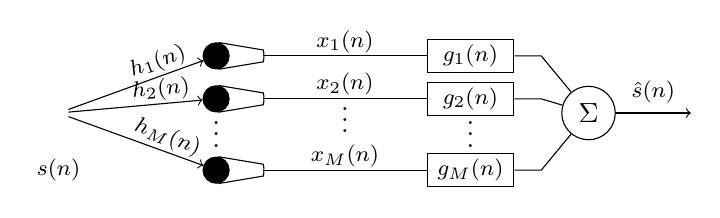
\begin{tikzpicture}
    % Adjustments
    \def\micd{.1cm}                % mic diameter
    \def\micl{.6cm}                % mic length
    \def\micw{.15cm}                % mic width
    \def\micbend{10}               % mic bottom bend
    \def\micdistance{.2cm}         % distance between microphones
    \def\filterdistance{2.5cm}     % distance between microphone and filter
    \def\filteroutline{.9cm}       % length of line which gets out of filter
    \def\sumdistance{1.5cm}        % distance of sum node to the filter
    \def\sumoutline{1cm}           % length of line which gets out of sum
    \def\headdistance{2cm}         % distance between microphone and head

    % Styles
    \tikzset{%
      mic head/.style={fill=black,draw=black,circle,minimum size=\micd},
      filter/.style={draw,minimum width=1.1cm,inner sep=2pt},
      sum/.style={draw,circle},
      xlabel/.style={inner sep=1pt,above,midway},
      sumlabel/.style={xlabel},
      hlabel/.style={xlabel,sloped,pos=.7},
      head/.style={font=\Large}
    }

    % Draw Microphones
    \begin{scope}[start chain=going below,every node/.style={on chain},node distance=\micdistance]
      \node[mic head] (mic1) {};
      \node[mic head] (mic2) {};
      \node[mic head,yshift=-1.8*\micdistance] (mic3) {};
    \end{scope}
    \node[yshift=3pt] at ($(mic2)!.5!(mic3)$) {$\vdots$};

    \foreach \m in {1,2,3} {%
      \coordinate (m1) at ($(mic\m)+(\micl,\micw/2)$);
      \coordinate (m2) at ($(mic\m)+(\micl,-\micw/2)$);
      \draw (tangent cs:node=mic\m,point={(m1)},solution=1) -- (m1) to[bend left=\micbend] (m2) -- (tangent cs:node=mic\m,point={(m2)},solution=2);
    }

    % Draw Filter
    \foreach \m/\i in {1/1,2/2,3/M} {%
      \node[filter,right=\filterdistance of mic\m] (filter\m) {\footnotesize $g_{\i}(n)$};
      \draw ($(mic\m)+(\micl,0)$) to node[xlabel] (x\m) {\footnotesize $x_{\i}(n)$} (filter\m);
    }
    \node[yshift=3pt] at ($(filter2)!.5!(filter3)$) {$\vdots$};
    \node[yshift=3pt] at ($(x2)!.5!(x3)$) {$\vdots$};
    % Sum Node
    \node[sum] (sum) at ($(filter1)!.5!(filter3)+(\sumdistance,0)$) {$\Sigma$};
    \draw[->] (sum) -- node[above] {\footnotesize $\hat{s}(n)$} ++(1.3,0);
    % Connect filter with sum
    \foreach \m in {1,2,3} {%
      \draw (filter\m) -- ++(\filteroutline,0) -- (sum);
    }

    % Head
    \node[head] (head) at ($(mic1)!.5!(mic3)-(\headdistance,0)$) {\PHtattooedHead};
    \node[fill=white,minimum width=4.8pt,minimum height=5.7pt,inner sep=0pt] at ($(head.center)+(2.3pt,-2.5pt)$) {};
    \node at ($(head.center)+(0.0pt,-20.5pt)$) {\footnotesize $s(n)$};
    % Connect head with mics
    \foreach \m/\i in {1/1,2/2,3/M} {%
      \draw[->] (head) -- node[hlabel] {\footnotesize $h_{\i}(n)$} (mic\m);
    }
  \end{tikzpicture}
  \caption{Multichannel equalization system}
  \label{fig: acsys}
\end{figure}
Given inverse filters $\mathbf{g}_m$ of length $L_g$, i.e. $\mathbf{g}_m = [g_m(0) \; g_m(1) \; \ldots$ $ g_m(L_g-1)]^T$, $m = 1, \; \ldots, \; M$,
the output of the multichannel equalization system is equal to
\begin{equation}  
  \hat{s}(n) = s(n) \ast \sum_{m=1}^{M} h_m(n) \ast g_m(n) = s(n) \ast c(n),
\end{equation}
where $\ast$ denotes the convolution operation, $n$ is the time index, and the  $(L_h+L_g-1)$-dimensional vector $\mathbf{c}$ is defined as the \emph{equalized impulse response} (EIR) between the source and the output signal.
Using the concatenated convolution matrix $\mathbf{H}$ and the stacked vector of inverse filters $\mathbf{g}$, i.e.
\begin{eqnarray}
  \mathbf{H}  &=&  \left[\mathbf{H}_1 \; \mathbf{H}_2 \; \ldots \; \mathbf{H}_M \right]_{(L_h+L_g-1)\times ML_g} \\
  \mathbf{g}  &=& \left[\mathbf{g}_1^T \; \mathbf{g}_2^T \; \ldots \; \mathbf{g}_M^T \right]_{ML_g \times 1}^T,
\end{eqnarray}
with $\mathbf{H}_m$ the $(L_h+L_g-1)\times L_g$-dimensional convolution matrix of $\mathbf{h}_m$, the EIR can be expressed as
\begin{equation}
\label{eq: c}
\mathbf{c} = \mathbf{H} \mathbf{g}.
\end{equation}
Inverse filters $\mathbf{g}$ can then be constructed based on different design objectives for $\mathbf{c}$.

\smallskip \noindent \textit{MINT.} \enspace The multiple-input/output inverse theorem~\cite{Miyoshi_ITASS_1988} aims to recover the anechoic speech signal up to a delay $\tau$ by minimizing the least-squares cost function
\begin{equation}
\label{eq: cost_mint}
\boxed{J_{{}_{\rm MINT}}(\mathbf{g}) = \|\mathbf{H}\mathbf{g} - \mathbf{d}\|_2^2}
\end{equation}
with
\begin{equation}
  \mathbf{d} = [\underbrace{0 \; \ldots \; 0}_{\tau} \; 1 \; 0 \; \ldots \; 0 ]_{(L_h+L_g-1) \times 1}^T.
\end{equation}
It has been shown in~\cite{Miyoshi_ITASS_1988} that when the RIRs do not share any common zeros in the $z$-plane and when $L_g \geq \lceil{\frac{L_h-1}{M-1}\rceil}$, inverse filters that perfectly equalize the channel can be computed as
\begin{equation}
  \mathbf{g}_{{}_{\rm MINT}} = \mathbf{H}^+\mathbf{d},
\end{equation}
where $\{\cdot\}^+$ denotes the Moore-Penrose pseudo-inverse. 
However, in practice the estimated room impulse responses generally differ from the real ones, and the application of the MINT inverse filters leads to large distortions in the output signal.

Experimental investigations e.g. in~\cite{Zhang_IWAENC_2010,Kodrasi_ICASSP_2012} have shown that techniques aiming only at partial equalization such as the ones described below are significantly more robust in the presence of channel estimation errors.

\smallskip \noindent \textit{P-MINT.} \enspace The partial multichannel equalization approach based on MINT aims at setting the reverberant tail of the EIR to $0$, while still controlling the remaining taps corresponding to the direct path and early reflections~\cite{Kodrasi_ICASSP_2012}. 
To accomplish this objective, the first part of one of the estimated RIRs is used as the target response in~(\ref{eq: cost_mint}), i.e.  
\begin{equation}
\boxed{J_{{}_{\rm P-MINT}}(\mathbf{g}) = \|{\mathbf{H}}\mathbf{g} - {\mathbf{h}}_p^{\rm d}\|_2^2}
\end{equation}
where
\begin{equation}
\small
\mathbf{h}_{p}^{\rm d} = [\underbrace{0\phantom{\rlap{$(L_d-1)$}} \ldots 0 }_{\tau} \underbrace{h_p(0) \ldots h_p(L_d-1)}_{L_d} 0 \ldots 0 ]_{(L_h+L_g-1) \times 1}^{T},
\end{equation}
with $p \in \{1, \; \ldots, \; M\}$ and $L_d$ denoting the length of the direct path and early reflections~(in number of samples), which is typically considered to be between $50$ and $80$~ms.
Inverse filters that partially equalize the channel can then be computed as
\begin{equation}  
\label{eq: Pmintsol}  
\mathbf{g}_{{}_{\rm P-MINT}} = {\mathbf{H}}^{+}{\mathbf{h}}_p^{\rm d}.
\end{equation}  

\smallskip \noindent \textit{RMCLS.} \enspace The relaxed multichannel least-squares technique~\cite{Zhang_IWAENC_2010} aims at setting the reverberant tail of the EIR to $0$, while putting no constraints on the direct path and early reflections. 
This can be achieved by introducing a weighting matrix $\mathbf{W}$ in the least-squares cost function in~(\ref{eq: cost_mint}), i.e.
\begin{equation}
\label{eq: rmcls_cost}
\boxed{J_{{}_{\rm RMCLS}}(\mathbf{g}) = \|\mathbf{W}({\mathbf{H}}\mathbf{g} - \mathbf{d})\|_2^2}
\end{equation}
with $\mathbf{W} = {\rm diag}\{\mathbf{w}\}$, and
\begin{equation}
\mathbf{w} = [\underbrace{1 \; \ldots \; 1}_{\tau} \; \underbrace{1 \; 0 \; \ldots \; 0}_{L_d} \; 1 \; \ldots 1]_{(L_h+L_g-1) \times 1}^{T},
\end{equation}
Inverse filters minimizing~(\ref{eq: rmcls_cost}) can be computed as
\begin{equation}
\mathbf{g}_{{}_{\rm RMCLS}}= (\mathbf{W}{\mathbf{H}})^{+}\mathbf{W}\mathbf{d}.
\end{equation}

\smallskip \noindent \textit{CS.} \enspace Channel shortening aims at suppressing the reverberant tail by maximizing the ratio of the energy in the first $L_d$ taps and in the remaining taps of the EIR~\cite{Zhang_IWAENC_2010}. 
This optimization problem is expressed in terms of a generalized Rayleigh quotient maximization problem, i.e.
\begin{equation}
\label{eq: cost_cs}
\boxed{J_{{}_{\rm CS}}(\mathbf{g})= \frac{\mathbf{g}^T {\mathbf{B}} \mathbf{g}}{\mathbf{g}^T {\mathbf{A}} \mathbf{g}}}
\end{equation}
where
\begin{eqnarray}
\label{eq: wincs}
{\mathbf{B}} & = & {\mathbf{H}}^{T} {\rm diag}\{\mathbf{w}_d \}^T {\rm diag}\{\mathbf{w}_d \}{\mathbf{H}}  \\
{\mathbf{A}} & = & {\mathbf{H}}^{T} {\rm diag}\{\mathbf{w}_u \}^T {\rm diag}\{\mathbf{w}_u \}{\mathbf{H}}  \\
\mathbf{w}_d & = & [\underbrace{0 \; \ldots \; 0}_{\tau} \; \underbrace{1 \; \ldots \; 1}_{L_{d}}\; 0\; \ldots\; 0]_{(L_h+L_g-1) \times 1}^{T}  \\
\mathbf{w}_u & = & \mathbf{1}_{(L_h+L_g-1)\times 1} - \mathbf{w}_d.
\end{eqnarray}
Maximizing~(\ref{eq: cost_cs}) is equivalent to solving the generalized eigenvalue problem $\mathbf{B} \mathbf{g} = \lambda \mathbf{A} \mathbf{g}$, where the optimal filter $\mathbf{g}$ is the generalized eigenvector corresponding to the largest generalized eigenvalue.
However, since multiple eigenvectors maximize~(\ref{eq: cost_cs}), in~\cite{Zhang_IWAENC_2010} it has been proposed to use the eigenvector leading to the minimum $l_2$-norm EIR.
\vspace{-0.1cm}

\section{Regularization in Acoustic Multichannel Equalization}
\vspace{-0.2cm}

The estimated room impulse responses $\hat{h}_m(n)$ generally differ from the real ones~(e.g. due to the sensitivity of blind system identification methods to interfering noise), i.e.
\begin{equation}
\hat{h}_m(n) = h_m(n)+\epsilon_m(n),
\end{equation}
with $\epsilon_m(n)$ the estimation error.
When equalization filters are designed using these erroneous estimates, the output signal is equal to
\begingroup
\fontsize{7.7pt}{7.7pt}\selectfont
\begin{align}
\hat{s}(n)  & =\!\! \sum_{m=1}^M s(n) \ast h_m(n) \ast g_m(n) \\
& = \!\! \sum_{m=1}^M s(n) \ast \left[\hat{h}_m(n) - \epsilon_m(n)\right] \ast g_m(n) \\
\label{eq: 2}
 &  = \!\! \sum_{m=1}^M s(n) \ast \hat{h}_m(n) \ast g_m(n) - \sum_{m=1}^M s(n) \ast \epsilon_m(n) \ast g_m(n).
\end{align}
\endgroup

\noindent
The first term in~(\ref{eq: 2}) represents the desired speech signal whereas the second term represents the distortion introduced due to the channel estimation errors. 
When the designed inverse filters have low energy, then the value of the distortion term is also small.
To decrease the energy of the inverse filters, a regularization term $\delta \|\mathbf{g}\|_2^2$ can be incorporated in all the previously discussed cost functions, with $\delta$ a regularization parameter controlling the weight given to the minimization of the energy of the inverse filters.

\smallskip \noindent \textit{Regularized MINT.} \enspace In the regularized MINT approach in~\cite{Hikichi_EURASIP_2007}, the cost function in~(\ref{eq: cost_mint}) is extended to
\begin{equation}
\label{eq: cost_rmint}
\boxed{J_{{}_{\rm RMINT}}(\mathbf{g}) = \|\mathbf{H}\mathbf{g} - \mathbf{d}\|_2^2 + \delta \|\mathbf{g} \|_2^2} 
\end{equation}
By setting the gradient of~(\ref{eq: cost_rmint}) to $0$, % i.e.
% \begin{equation}
% \frac{\partial J_{{}_{\rm RMINT}}(\mathbf{g})}{\partial \mathbf{g}} = 2\mathbf{H}^T\mathbf{H}\mathbf{g} - 2\mathbf{H}^T\mathbf{d} + 2 \delta \mathbf{g}  = 0,
% \end{equation}
the inverse filters can be computed as
\begin{equation}
\label{eq: rmint_sol}
\mathbf{g}_{{}_{\rm RMINT}}  = (\mathbf{H}^T\mathbf{H}+\delta \mathbf{I})^{-1}\mathbf{H}^{T}\mathbf{d},
\end{equation}
where $\mathbf{I}$ is the $(ML_g) \times (ML_g)$-dimensional identity matrix. 

\smallskip \noindent \textit{Regularized P-MINT.} \enspace Similarly to the regularized least-squares approach for MINT, the P-MINT cost function is extended to~\cite{Kodrasi_ICASSP_2012}
\begin{equation}
\label{eq: cost_rpmint}
\boxed{J_{{}_{\rm RP-MINT}}(\mathbf{g}) = \|\mathbf{H}\mathbf{g} - \mathbf{h}_p^{\rm d}\|_2^2 + \delta \|\mathbf{g} \|_2^2}
\end{equation}
Minimizing~(\ref{eq: cost_rpmint}) yields the regularized P-MINT inverse filters
\begin{equation}
\mathbf{g}_{{}_{\rm RP-MINT}}  = (\mathbf{H}^T\mathbf{H}+\delta \mathbf{I})^{-1}\mathbf{H}^{T}\mathbf{h}_p^{\rm d}.
\end{equation}
It has been shown in~\cite{Kodrasi_ICASSP_2012} that the regularized P-MINT approach achieves a significantly higher suppression of the reverberant tail in comparison to P-MINT.
Hence, in the following we propose to also incorporate the regularization term $\delta \|\mathbf{g} \|_2^2$ into the RMCLS and CS equalization techniques.

\smallskip \noindent \textit{Regularized RMCLS.} \enspace Since RMCLS is also a least-squares approach, the incorporation of a regularization parameter can be done similarly as before, i.e.
\begin{equation}
\label{eq: cost_rrmcls}
\boxed{J_{{}_{\rm RRMCLS}}(\mathbf{g}) =  \|\mathbf{W}({\mathbf{H}}\mathbf{g} - \mathbf{d})\|_2^2 + \delta \|\mathbf{g} \|_2^2}
\end{equation}
By setting the derivative of~(\ref{eq: cost_rrmcls}) to $0$, the regularized RMCLS inverse filters can be computed as
\begin{equation}
\mathbf{g}_{{}_{\rm RRMCLS}}  = [(\mathbf{W}\mathbf{H})^T(\mathbf{W}\mathbf{H}) + \delta \mathbf{I}]^{-1} (\mathbf{W}\mathbf{H})^T \mathbf{W}\mathbf{d.}
\end{equation}

\smallskip \noindent \textit{Regularized CS.} \enspace In order to integrate a regularization parameter in channel shortening, we reformulate the maximization problem in~(\ref{eq: cost_cs}) in terms of a generalized Rayleigh quotient minimization problem, such that the regularized CS cost function to be minimized can be defined as
\begin{equation}
\label{eq: cost_rcs}
\boxed{J_{{}_{\rm RCS}}(\mathbf{g})= \frac{\mathbf{g}^T {\mathbf{A}} \mathbf{g}}{\mathbf{g}^T {\mathbf{B}} \mathbf{g}} + \delta \|\mathbf{g} \|_2^2}
\end{equation}
However, since no analytical solution to~(\ref{eq: cost_rcs}) exists, we have used a non-linear optimization technique for minimizing this cost function.
In order to improve the numerical robustness and the convergence speed of the optimization technique, the gradient
\begin{equation}
\frac{\partial J_{{}_{\rm RCS}}(\mathbf{g})}{\partial \mathbf{g}} = 2 \frac{(\mathbf{g}^T \mathbf{B} \mathbf{g})\mathbf{A}\mathbf{g} - (\mathbf{g}^T \mathbf{A} \mathbf{g})\mathbf{B}\mathbf{g} }{(\mathbf{g}^T \mathbf{B} \mathbf{g})^2} + 2 \delta \mathbf{g},
\end{equation}
and the Hessian
\begin{equation}
\begin{split}
& \frac{\partial ^2 J_{{}_{\rm RCS}}(\mathbf{g})}{\partial^2 \mathbf{g}}  = \\
& 2 \left[ \frac{(\mathbf{g}^T \mathbf{B} \mathbf{g}) \mathbf{A} - (\mathbf{g}^T \mathbf{A} \mathbf{g}) \mathbf{B} + 2 ( \mathbf{A} \mathbf{g} \mathbf{g}^T \mathbf{B} - \mathbf{B} \mathbf{g} \mathbf{g}^T \mathbf{A})}{(\mathbf{g}^T \mathbf{B}\mathbf{g})^2} \right] \\
& -  4 \frac{[(\mathbf{g}^T\mathbf{B}\mathbf{g})\mathbf{A}\mathbf{g} - (\mathbf{g}^T\mathbf{A}\mathbf{g})\mathbf{B}\mathbf{g}] \mathbf{g}^T \mathbf{B}}{(\mathbf{g}^T\mathbf{B}\mathbf{g})^3} + 2 \delta \mathbf{I},
\end{split}
\end{equation}
can be provided. 
It should be noted that this approach is sensitive to the initial vector provided to the numerical optimization algorithm, sometimes getting stuck into local minima.
However, in an attempt to find optimal inverse filters, we have analyzed a set of initial vectors and have selected the optimal solution as the one leading to the highest perceptual sound quality~(cf. Section~\ref{sec: exp}).

Increasing the parameter $\delta$ in all the regularized techniques presented above decreases the norm of $\mathbf{g}$, making the inverse filter less sensitive to estimation errors of the RIRs. 
However, increasing this parameter also reduces the equalization performance with respect to the true RIRs, resulting in a trade-off between performance for perfectly estimated room impulse responses and robustness in the presence of channel estimation errors.

\vspace{-0.1cm}
\section{Experimental Results}
\label{sec: exp}
\vspace{-0.2cm}

To investigate the effectiveness of regularization for the considered equalization techniques, we have used a measured $2$-channel system with reverberation time $T_{60} \approx 600$~ms as the true system to be equalized. 
In order to generate the estimated room impulse responses, the actual RIRs are perturbed by adding scaled white noise as proposed in~\cite{Cho_ITSA_1999}, i.e. $\hat{h}_m(n) = h_m(n) + {\epsilon}_m(n)h_m(n)$, where ${\epsilon}_m(n)$ is an uncorrelated Gaussian noise sequence with zero mean and $-33$~dB variance, such that the channel mismatch
\begin{equation}
  E_m = 10 \log_{10} \frac{\|\mathbf{h}_m-\hat{\mathbf{h}}_m\|_2^2}{\|\mathbf{h}_m\|_2^2} = -33{\; \rm dB},
\end{equation}
is generated\footnote{Several other channel mismatch values have been investigated which lead to similar conclusions as the ones derived here. 
However, these results have been omitted due to space constraints.}.
In addition, the sampling frequency is $f_s = 16$~kHz and the simulation parameters are set to $L_h = 2000$, $L_g = 1999$, and $\tau = 0$.
The considered desired window lengths are $10$~ms, $20$~ms, $30$~ms, $40$~ms, and $50$~ms.
Furthermore, the target response in P-MINT is chosen as the direct path and early reflections of the first estimated channel, i.e. $\hat{\mathbf{h}}_1^{\rm d}$.

The reverberant tail suppression is evaluated using the \emph{energy decay curve}~(EDC) of the EIR, defined as
\begin{equation}
\small
\hspace{-0.01cm} \hbox{EDC}(n)\! = \!10 \log_{10}\frac{1}{\|\mathbf{c}\|_2^2}\!\!\!\!\!\sum_{i=n}^{L_h+L_g-2}\!\!\!\!\!c^2(i), \; n \!=\! 0,  \ldots,  L_h\!+\!L_g\!-\!2. \hspace{-0.06cm}
\end{equation}
To evaluate the perceptual sound quality we have used the objective speech quality measure PESQ~\cite{PESQ} with $s(n) \ast h_1^{\rm d}(n)$ as reference signal.
It has been shown in~\cite{Goetze_AES_2010} that measures relying on auditory models such as PESQ exhibit the highest correlation with subjective listening tests when evaluating the quality of dereverberated speech.

As regularization parameter $\delta$ in all regularized approaches, we have considered $ \delta \in \{0, \; 10^{-9}, \;10^{-8}, \;  \ldots, \; 10^{-1} \}$,
and the optimal parameter for each equalization technique is selected as the one leading to the highest perceptual sound quality, i.e. PESQ score. 
Such a selection procedure for the regularization parameter yields the EDCs depicted in Fig.~\ref{fig: EDCs} for a desired window length $L_d = 0.04 f_s$. 
As can be observed in this figure, the regularized MINT approach fails to equalize the channel, leading to an EDC that is only slightly lower than the one of the original RIR. 
On the contrary, all the partial multichannel equalization techniques are significantly more robust, leading to a similar performance in terms of the reverberant tail suppression. 
While the regularized RMCLS approach appears to yield the highest suppression, also the decay rates of the EDCs obtained through regularized CS and regularized P-MINT are satisfactory, with their reverberant tails being below audible levels. 

\begin{figure}[t!]
\centering
\includegraphics[scale=0.61]{EDC_sys_5_Cm_-33_Ld_640}
\vspace{-0.8cm}
\caption{EDC obtained using regularized CS, regularized P-MINT, regularized RMCLS, regularized MINT, and EDC of $\mathbf{h}_1$ for the desired window length $\frac{L_d \times 10^{3}}{f_s} = 40$~ms}
\vspace{-0.5cm}
\label{fig: EDCs}
\end{figure}
Since different EIRs leading to different perceptual sound quality may have very similar EDCs~(which is the case for all the partial multichannel equalization techniques in this simulation), we have also evaluated the perceptual sound quality using PESQ with $s(n) \ast h_1^{\rm d}(n)$ as the reference signal for each value of the desired window length $L_d$.
In order to determine the effectiveness of incorporating a regularization parameter, we have computed the difference between the PESQ scores obtained with regularization and without regularization.
This difference for all considered techniques and desired window lengths is presented in Table~\ref{tbl: deltapesq}.
Additionally, the average change in PESQ over all considered $L_d$ values is also presented.
It can be noticed that regularization is particularly useful for the P-MINT and CS approaches, leading to an average improvement of the PESQ score of $1.37$ and $1.08$, respectively.
Furthermore, also the regularized MINT technique leads to a higher performance as compared to MINT, whereas no meaningful advantage of incorporating a regularization term for RMCLS can be noticed.

Finally, in order to compare the perceptual sound quality of the different considered techniques, Fig.~\ref{fig: PESQ} depicts the PESQ scores for all equalization approaches as a function of the desired window length $L_d$.
It can be seen that the regularized MINT approach leads to a very similar perceptual quality as the original reverberant signal, whereas a significant improvement is achieved when using the partial equalization techniques.
As illustrated in this figure, similar performance is achieved by all partial equalization techniques when the desired window length is $10$~ms, while for $20$~ms, $30$~ms, $40$~ms, and $50$~ms the regularized P-MINT approach yields the highest perceptual sound quality.

\vspace{-0.1cm}
\section{Conclusion}
\vspace{-0.2cm}

In this paper, we have presented an extension to the recently proposed relaxed multichannel least-squares and channel shortening techniques by incorporating a regularization term in the inverse filter design.
Furthermore, we have extensively investigated the effectiveness of regularization in terms of reverberant tail suppression and perceptual sound quality for all equalization techniques, i.e. MINT, P-MINT, RMCLS, and CS.
Simulation results show that regularization is particularly important for P-MINT, CS, and MINT whereas for RMCLS no significant performance improvement is achieved. 
Furthermore, experimental results demonstrate that the regularized P-MINT approach leads to the highest quality of perceived speech in the presence of channel estimation errors.

%In order to compare these techniques in terms of the quality of perceived speech.
% References should be produced using the bibtex program from suitable
% BiBTeX files (here: strings, refs, manuals). The IEEEbib.bst bibliography
% style file from IEEE produces unsorted bibliography list.
% -------------------------------------------------------------------------
\bibliographystyle{IEEEtran}
\bibliography{refs}

\begin{table}[t!]
\footnotesize
\centering
\caption{Improvement in PESQ score when incorporating a regularization parameter in all considered techniques for several desired window lengths $L_d$}
\label{tbl: deltapesq}
 \begin{tabular}{|l|r|r|r|r|r|r|}
   \hline
   {\footnotesize $L_d \times \frac{10^{3}}{f_s}$~[ms] }& $10$ & $20$ & $30$ & $40$ & $50$ & Average \\ \hline
   MINT & $0.38$ & $0.31$ & $0.33$ & $0.37$ & $0.31$ & $0.34$ \\ \hline
   P-MINT & $0.71$ & $\bf{1.61}$ & $\bf{1.87}$ & $\bf{2.10}$ & $\bf{0.55}$ & $\bf{1.37}$ \\ \hline
   RMCLS & $0.00$ & $0.02$ & $0.04$ & $0.00$ & $0.00$ & $0.01$ \\ \hline
   CS & $\bf{1.41}$ & $1.41$ & $1.04$ & $1.53$ & $0.00$ & $1.08$ \\ \hline
\end{tabular}
\end{table}
\begin{figure}[t!]
\centering
\includegraphics[scale=0.61]{PESQreg_sys_5_Cm_-33}
\vspace{-0.8cm}
\caption{PESQ score of the reverberant signal and PESQ score of the system's output obtained using regularized CS, regularized P-MINT, regularized RMCLS, and regularized MINT for several considered desired window lengths $L_d$}
\vspace{-0.5cm}
\label{fig: PESQ}
\end{figure}
\end{document}
